% Options for packages loaded elsewhere
\PassOptionsToPackage{unicode}{hyperref}
\PassOptionsToPackage{hyphens}{url}
\PassOptionsToPackage{dvipsnames,svgnames,x11names}{xcolor}
%
\documentclass[
  b5paper,
  DIV=11,
  numbers=noendperiod]{scrreprt}

\usepackage{amsmath,amssymb}
\usepackage{iftex}
\ifPDFTeX
  \usepackage[T1]{fontenc}
  \usepackage[utf8]{inputenc}
  \usepackage{textcomp} % provide euro and other symbols
\else % if luatex or xetex
  \usepackage{unicode-math}
  \defaultfontfeatures{Scale=MatchLowercase}
  \defaultfontfeatures[\rmfamily]{Ligatures=TeX,Scale=1}
\fi
\usepackage{lmodern}
\ifPDFTeX\else  
    % xetex/luatex font selection
\fi
% Use upquote if available, for straight quotes in verbatim environments
\IfFileExists{upquote.sty}{\usepackage{upquote}}{}
\IfFileExists{microtype.sty}{% use microtype if available
  \usepackage[]{microtype}
  \UseMicrotypeSet[protrusion]{basicmath} % disable protrusion for tt fonts
}{}
\makeatletter
\@ifundefined{KOMAClassName}{% if non-KOMA class
  \IfFileExists{parskip.sty}{%
    \usepackage{parskip}
  }{% else
    \setlength{\parindent}{0pt}
    \setlength{\parskip}{6pt plus 2pt minus 1pt}}
}{% if KOMA class
  \KOMAoptions{parskip=half}}
\makeatother
\usepackage{xcolor}
\setlength{\emergencystretch}{3em} % prevent overfull lines
\setcounter{secnumdepth}{3}
% Make \paragraph and \subparagraph free-standing
\makeatletter
\ifx\paragraph\undefined\else
  \let\oldparagraph\paragraph
  \renewcommand{\paragraph}{
    \@ifstar
      \xxxParagraphStar
      \xxxParagraphNoStar
  }
  \newcommand{\xxxParagraphStar}[1]{\oldparagraph*{#1}\mbox{}}
  \newcommand{\xxxParagraphNoStar}[1]{\oldparagraph{#1}\mbox{}}
\fi
\ifx\subparagraph\undefined\else
  \let\oldsubparagraph\subparagraph
  \renewcommand{\subparagraph}{
    \@ifstar
      \xxxSubParagraphStar
      \xxxSubParagraphNoStar
  }
  \newcommand{\xxxSubParagraphStar}[1]{\oldsubparagraph*{#1}\mbox{}}
  \newcommand{\xxxSubParagraphNoStar}[1]{\oldsubparagraph{#1}\mbox{}}
\fi
\makeatother

\usepackage{color}
\usepackage{fancyvrb}
\newcommand{\VerbBar}{|}
\newcommand{\VERB}{\Verb[commandchars=\\\{\}]}
\DefineVerbatimEnvironment{Highlighting}{Verbatim}{commandchars=\\\{\}}
% Add ',fontsize=\small' for more characters per line
\usepackage{framed}
\definecolor{shadecolor}{RGB}{241,243,245}
\newenvironment{Shaded}{\begin{snugshade}}{\end{snugshade}}
\newcommand{\AlertTok}[1]{\textcolor[rgb]{0.68,0.00,0.00}{#1}}
\newcommand{\AnnotationTok}[1]{\textcolor[rgb]{0.37,0.37,0.37}{#1}}
\newcommand{\AttributeTok}[1]{\textcolor[rgb]{0.40,0.45,0.13}{#1}}
\newcommand{\BaseNTok}[1]{\textcolor[rgb]{0.68,0.00,0.00}{#1}}
\newcommand{\BuiltInTok}[1]{\textcolor[rgb]{0.00,0.23,0.31}{#1}}
\newcommand{\CharTok}[1]{\textcolor[rgb]{0.13,0.47,0.30}{#1}}
\newcommand{\CommentTok}[1]{\textcolor[rgb]{0.37,0.37,0.37}{#1}}
\newcommand{\CommentVarTok}[1]{\textcolor[rgb]{0.37,0.37,0.37}{\textit{#1}}}
\newcommand{\ConstantTok}[1]{\textcolor[rgb]{0.56,0.35,0.01}{#1}}
\newcommand{\ControlFlowTok}[1]{\textcolor[rgb]{0.00,0.23,0.31}{\textbf{#1}}}
\newcommand{\DataTypeTok}[1]{\textcolor[rgb]{0.68,0.00,0.00}{#1}}
\newcommand{\DecValTok}[1]{\textcolor[rgb]{0.68,0.00,0.00}{#1}}
\newcommand{\DocumentationTok}[1]{\textcolor[rgb]{0.37,0.37,0.37}{\textit{#1}}}
\newcommand{\ErrorTok}[1]{\textcolor[rgb]{0.68,0.00,0.00}{#1}}
\newcommand{\ExtensionTok}[1]{\textcolor[rgb]{0.00,0.23,0.31}{#1}}
\newcommand{\FloatTok}[1]{\textcolor[rgb]{0.68,0.00,0.00}{#1}}
\newcommand{\FunctionTok}[1]{\textcolor[rgb]{0.28,0.35,0.67}{#1}}
\newcommand{\ImportTok}[1]{\textcolor[rgb]{0.00,0.46,0.62}{#1}}
\newcommand{\InformationTok}[1]{\textcolor[rgb]{0.37,0.37,0.37}{#1}}
\newcommand{\KeywordTok}[1]{\textcolor[rgb]{0.00,0.23,0.31}{\textbf{#1}}}
\newcommand{\NormalTok}[1]{\textcolor[rgb]{0.00,0.23,0.31}{#1}}
\newcommand{\OperatorTok}[1]{\textcolor[rgb]{0.37,0.37,0.37}{#1}}
\newcommand{\OtherTok}[1]{\textcolor[rgb]{0.00,0.23,0.31}{#1}}
\newcommand{\PreprocessorTok}[1]{\textcolor[rgb]{0.68,0.00,0.00}{#1}}
\newcommand{\RegionMarkerTok}[1]{\textcolor[rgb]{0.00,0.23,0.31}{#1}}
\newcommand{\SpecialCharTok}[1]{\textcolor[rgb]{0.37,0.37,0.37}{#1}}
\newcommand{\SpecialStringTok}[1]{\textcolor[rgb]{0.13,0.47,0.30}{#1}}
\newcommand{\StringTok}[1]{\textcolor[rgb]{0.13,0.47,0.30}{#1}}
\newcommand{\VariableTok}[1]{\textcolor[rgb]{0.07,0.07,0.07}{#1}}
\newcommand{\VerbatimStringTok}[1]{\textcolor[rgb]{0.13,0.47,0.30}{#1}}
\newcommand{\WarningTok}[1]{\textcolor[rgb]{0.37,0.37,0.37}{\textit{#1}}}

\providecommand{\tightlist}{%
  \setlength{\itemsep}{0pt}\setlength{\parskip}{0pt}}\usepackage{longtable,booktabs,array}
\usepackage{calc} % for calculating minipage widths
% Correct order of tables after \paragraph or \subparagraph
\usepackage{etoolbox}
\makeatletter
\patchcmd\longtable{\par}{\if@noskipsec\mbox{}\fi\par}{}{}
\makeatother
% Allow footnotes in longtable head/foot
\IfFileExists{footnotehyper.sty}{\usepackage{footnotehyper}}{\usepackage{footnote}}
\makesavenoteenv{longtable}
\usepackage{graphicx}
\makeatletter
\def\maxwidth{\ifdim\Gin@nat@width>\linewidth\linewidth\else\Gin@nat@width\fi}
\def\maxheight{\ifdim\Gin@nat@height>\textheight\textheight\else\Gin@nat@height\fi}
\makeatother
% Scale images if necessary, so that they will not overflow the page
% margins by default, and it is still possible to overwrite the defaults
% using explicit options in \includegraphics[width, height, ...]{}
\setkeys{Gin}{width=\maxwidth,height=\maxheight,keepaspectratio}
% Set default figure placement to htbp
\makeatletter
\def\fps@figure{htbp}
\makeatother

\usepackage{libertine}
\addtokomafont{disposition}{\rmfamily}
\renewcommand{\ttdefault}{clmt}
       
\providecommand{\ped}[1]{_\textrm{#1}}
\providecommand{\ap}[1]{^\textrm{#1}}
\providecommand{\app}[1]{^\textrm{#1}}

\providecommand*{\angs}{\smash{\mathrm{\ring A}}}
\providecommand*{\celsius}{\mathrm{~\circ C}}
\providecommand*{\micro}{\mu}

\providecommand*{\unit}[1]{\textrm{\,#1}}

\providecommand{\E}{\mathrm{e}}
\providecommand{\I}{\mathrm{i}}
\providecommand{\sfrac}[2]{^{#1}/_{#2}}

\providecommand{\conc}[1]{\left[\mathrm{#1}\right]}


\providecommand{\command}[1]{\textsl{#1}}
\providecommand{\out}[1]{\begin{verbatim}#1\end{verbatim}}


\providecommand{\diff}{\mathrm{d}\,}


\providecommand*{\deriv}[3][]{% arguments: order of the derivative(optional), function, variable
	\frac{\diff^{#1}#2}{\diff #3^{#1}}}
\providecommand*{\pderiv}[3][]{% arguments: order of the derivative(optional), function, variable
	\frac{\partial^{#1}#2}
		{\partial #3^{#1}}}
  
\renewcommand{\vec}[1]{{\boldsymbol #1}}

\providecommand{\cov}[2]{\mathrm{Cov}\!\left(#1, #2\right)}
\providecommand{\var}[1]{\mathrm{Var}\!\left(#1\right)}

\providecommand{\mean}[1]{\overline{#1}}

\providecommand{\sd}[1]{\sigma\left(#1\right)}
\providecommand{\ev}[1]{\mathbb{E}\!\left(#1\right)}
\providecommand{\pr}[1]{\textrm{Pr}\!\left(#1\right)}
\KOMAoption{captions}{tableheading}
\makeatletter
\@ifpackageloaded{tcolorbox}{}{\usepackage[skins,breakable]{tcolorbox}}
\@ifpackageloaded{fontawesome5}{}{\usepackage{fontawesome5}}
\definecolor{quarto-callout-color}{HTML}{909090}
\definecolor{quarto-callout-note-color}{HTML}{0758E5}
\definecolor{quarto-callout-important-color}{HTML}{CC1914}
\definecolor{quarto-callout-warning-color}{HTML}{EB9113}
\definecolor{quarto-callout-tip-color}{HTML}{00A047}
\definecolor{quarto-callout-caution-color}{HTML}{FC5300}
\definecolor{quarto-callout-color-frame}{HTML}{acacac}
\definecolor{quarto-callout-note-color-frame}{HTML}{4582ec}
\definecolor{quarto-callout-important-color-frame}{HTML}{d9534f}
\definecolor{quarto-callout-warning-color-frame}{HTML}{f0ad4e}
\definecolor{quarto-callout-tip-color-frame}{HTML}{02b875}
\definecolor{quarto-callout-caution-color-frame}{HTML}{fd7e14}
\makeatother
\makeatletter
\@ifpackageloaded{bookmark}{}{\usepackage{bookmark}}
\makeatother
\makeatletter
\@ifpackageloaded{caption}{}{\usepackage{caption}}
\AtBeginDocument{%
\ifdefined\contentsname
  \renewcommand*\contentsname{Inhoudsopgave}
\else
  \newcommand\contentsname{Inhoudsopgave}
\fi
\ifdefined\listfigurename
  \renewcommand*\listfigurename{Lijst van figuren}
\else
  \newcommand\listfigurename{Lijst van figuren}
\fi
\ifdefined\listtablename
  \renewcommand*\listtablename{Lijst van tabellen}
\else
  \newcommand\listtablename{Lijst van tabellen}
\fi
\ifdefined\figurename
  \renewcommand*\figurename{Figuur}
\else
  \newcommand\figurename{Figuur}
\fi
\ifdefined\tablename
  \renewcommand*\tablename{Tabel}
\else
  \newcommand\tablename{Tabel}
\fi
}
\@ifpackageloaded{float}{}{\usepackage{float}}
\floatstyle{ruled}
\@ifundefined{c@chapter}{\newfloat{codelisting}{h}{lop}}{\newfloat{codelisting}{h}{lop}[chapter]}
\floatname{codelisting}{Listing}
\newcommand*\listoflistings{\listof{codelisting}{Lijst van listings}}
\usepackage{amsthm}
\theoremstyle{definition}
\newtheorem{exercise}{Oefening}[chapter]
\theoremstyle{remark}
\AtBeginDocument{\renewcommand*{\proofname}{Bewijs}}
\newtheorem*{remark}{Opmerking}
\newtheorem*{solution}{Oplossing}
\newtheorem{refremark}{Opmerking}[chapter]
\newtheorem{refsolution}{Oplossing}[chapter]
\makeatother
\makeatletter
\makeatother
\makeatletter
\@ifpackageloaded{caption}{}{\usepackage{caption}}
\@ifpackageloaded{subcaption}{}{\usepackage{subcaption}}
\makeatother
\newcounter{quartocallouttipno}
\newcommand{\quartocallouttip}[1]{\refstepcounter{quartocallouttipno}\label{#1}}

\ifLuaTeX
\usepackage[bidi=basic]{babel}
\else
\usepackage[bidi=default]{babel}
\fi
\babelprovide[main,import]{dutch}
% get rid of language-specific shorthands (see #6817):
\let\LanguageShortHands\languageshorthands
\def\languageshorthands#1{}
\ifLuaTeX
  \usepackage{selnolig}  % disable illegal ligatures
\fi
\usepackage{bookmark}

\IfFileExists{xurl.sty}{\usepackage{xurl}}{} % add URL line breaks if available
\urlstyle{same} % disable monospaced font for URLs
\hypersetup{
  pdftitle={Kwantitatieve Biologie},
  pdfauthor={Vakgroep Biologie, Universiteit Utrecht},
  pdflang={nl},
  colorlinks=true,
  linkcolor={blue},
  filecolor={Maroon},
  citecolor={Blue},
  urlcolor={Blue},
  pdfcreator={LaTeX via pandoc}}


\title{Kwantitatieve Biologie}
\author{Vakgroep Biologie, Universiteit Utrecht}
\date{2024-06-20}

\begin{document}
\maketitle

\renewcommand*\contentsname{Inhoudsopgave}
{
\hypersetup{linkcolor=}
\setcounter{tocdepth}{2}
\tableofcontents
}

\part{Inleiding}

\part{Basiswiskunde}

\begin{figure}

\centering{

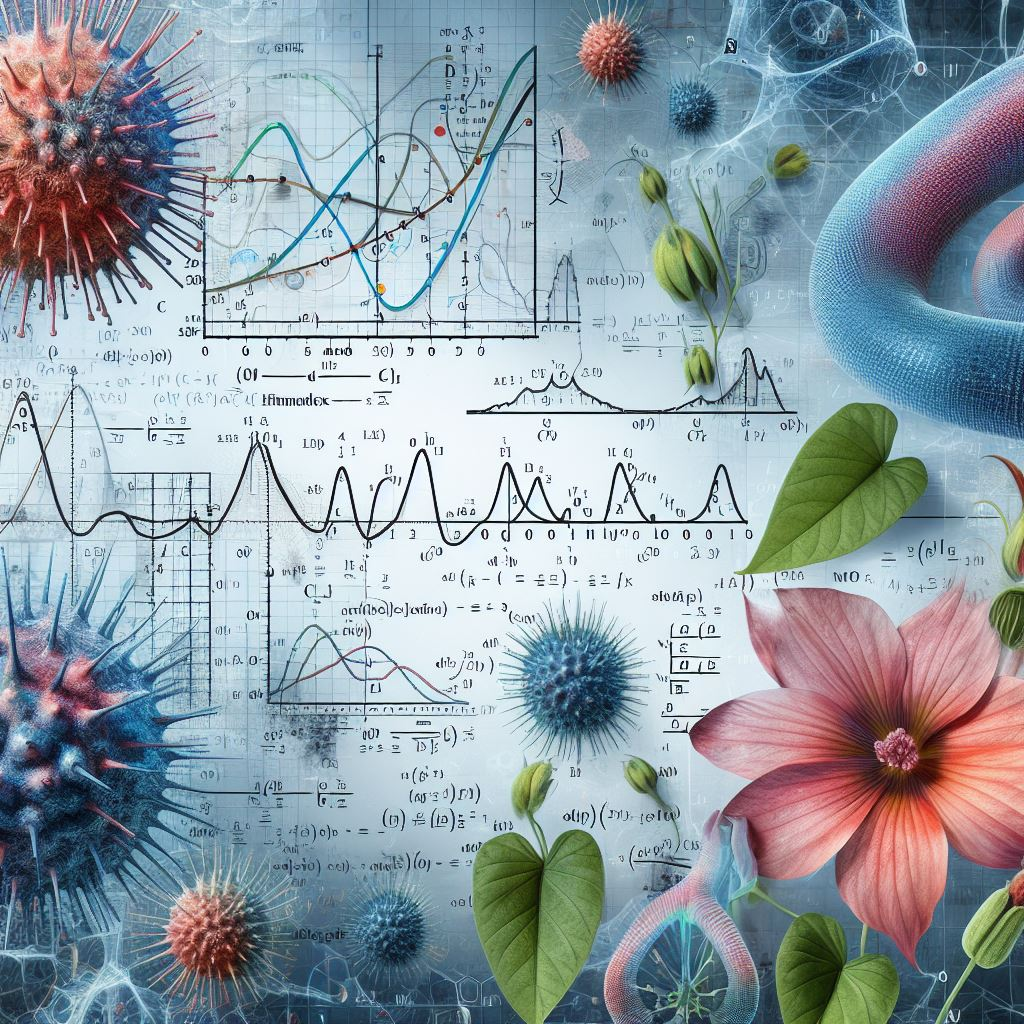
\includegraphics{Wiskunde/figuren/AI_mathematics.jpeg}

}

\caption{\label{fig-AI_mathematics}Wiskunde in de biologie; illustratie
gegenereerd door AI. (DALL-E 3, maart 2024)}

\end{figure}%

\chapter{Breuken}\label{breuken}

\bookmarksetup{startatroot}

\chapter{Voorbeelden van wat mogelijk is met
Quarto}\label{voorbeelden-van-wat-mogelijk-is-met-quarto}

\usepackage{libertine}
\addtokomafont{disposition}{\rmfamily}
\renewcommand{\ttdefault}{clmt}

\providecommand{\ped}[1]{_\textrm{#1}}
\providecommand{\ap}[1]{^\textrm{#1}}
\providecommand{\app}[1]{^\textrm{#1}}

\providecommand*{\angs}{\smash{\mathrm{\ring A}}}
\providecommand*{\celsius}{\mathrm{~\circ C}}
\providecommand*{\micro}{\mu}

\providecommand*{\unit}[1]{\textrm{\,#1}}

\providecommand{\E}{\mathrm{e}}
\providecommand{\I}{\mathrm{i}}
\providecommand{\sfrac}[2]{^{#1}/_{#2}}

\providecommand{\conc}[1]{\left[\mathrm{#1}\right]}

\providecommand{\command}[1]{\textsl{#1}}
\providecommand{\out}[1]{\begin{verbatim}#1\end{verbatim}}

\providecommand{\diff}{\mathrm{d}\,}

\providecommand*{\deriv}[3][]{% arguments: order of the derivative(optional), function, variable
    \frac{\diff^{#1}#2}{\diff #3^{#1}}}
\providecommand*{\pderiv}[3][]{% arguments: order of the derivative(optional), function, variable
    \frac{\partial^{#1}#2}
        {\partial #3^{#1}}}

\renewcommand{\vec}[1]{{\boldsymbol #1}}

\providecommand{\cov}[2]{\mathrm{Cov}\!\left(#1, #2\right)}
\providecommand{\var}[1]{\mathrm{Var}\!\left(#1\right)}

\providecommand{\mean}[1]{\overline{#1}}

\providecommand{\sd}[1]{\sigma\left(#1\right)}
\providecommand{\ev}[1]{\mathbb{E}\!\left(#1\right)}
\providecommand{\pr}[1]{\textrm{Pr}\!\left(#1\right)}

\section{Hoofdstuk}\label{hoofdstuk}

\subsection{Paragraaf binnen
hoofdstukje}\label{paragraaf-binnen-hoofdstukje}

\subsection{Plotjes maken in R}\label{plotjes-maken-in-r}

\begin{Shaded}
\begin{Highlighting}[]
\FunctionTok{library}\NormalTok{(ggplot2)}
\FunctionTok{library}\NormalTok{(tidyverse)}

\NormalTok{z\_values }\OtherTok{\textless{}{-}} \FunctionTok{seq}\NormalTok{(}\SpecialCharTok{{-}}\DecValTok{3}\NormalTok{, }\DecValTok{3}\NormalTok{, }\AttributeTok{by =} \FloatTok{0.01}\NormalTok{)}
\NormalTok{probabilities }\OtherTok{\textless{}{-}} \FunctionTok{dnorm}\NormalTok{(z\_values)}

\NormalTok{df }\OtherTok{\textless{}{-}} \FunctionTok{data.frame}\NormalTok{(}\AttributeTok{Z =}\NormalTok{ z\_values, }\AttributeTok{probability =}\NormalTok{ probabilities)}

\NormalTok{arrows }\OtherTok{\textless{}{-}} \FunctionTok{tibble}\NormalTok{(}
  \AttributeTok{x1 =} \FunctionTok{c}\NormalTok{(}\FloatTok{2.2}\NormalTok{), }
  \AttributeTok{x2 =} \FunctionTok{c}\NormalTok{(}\FloatTok{3.3}\NormalTok{),}
  \AttributeTok{y1 =} \FunctionTok{c}\NormalTok{(.}\DecValTok{02}\NormalTok{),}
  \AttributeTok{y2 =} \FunctionTok{c}\NormalTok{(}\FloatTok{0.15}\NormalTok{)}
\NormalTok{)}

\NormalTok{p }\OtherTok{\textless{}{-}} \FunctionTok{ggplot}\NormalTok{(df, }\FunctionTok{aes}\NormalTok{(}\AttributeTok{x =}\NormalTok{ Z, }\AttributeTok{y =}\NormalTok{ probability)) }\SpecialCharTok{+}
  \FunctionTok{geom\_line}\NormalTok{(}
    \AttributeTok{size =} \FloatTok{1.2}\NormalTok{,}
    \AttributeTok{color =} \StringTok{"\#e8601d"}
\NormalTok{    ) }\SpecialCharTok{+}
  \FunctionTok{geom\_ribbon}\NormalTok{(}
    \AttributeTok{data =} \FunctionTok{subset}\NormalTok{(df, Z }\SpecialCharTok{\textgreater{}=} \FloatTok{1.96}\NormalTok{), }
    \FunctionTok{aes}\NormalTok{(}\AttributeTok{ymax =}\NormalTok{ probability, }\AttributeTok{ymin =} \DecValTok{0}\NormalTok{), }
    \AttributeTok{fill =} \StringTok{"goldenrod"}\NormalTok{, }
    \AttributeTok{alpha =} \FloatTok{0.5}\NormalTok{) }\SpecialCharTok{+}
  \FunctionTok{geom\_vline}\NormalTok{(}
    \AttributeTok{xintercept =} \FloatTok{1.96}\NormalTok{, }
    \AttributeTok{linetype =} \StringTok{"dashed"}\NormalTok{, }
    \AttributeTok{color =} \StringTok{"black"}
\NormalTok{    ) }\SpecialCharTok{+}
  \FunctionTok{geom\_text}\NormalTok{(}
    \AttributeTok{x =} \FloatTok{0.6}\NormalTok{, }\AttributeTok{y =} \FloatTok{0.04}\NormalTok{, }
    \AttributeTok{label =} \FunctionTok{expression}\NormalTok{(}\FunctionTok{italic}\NormalTok{(Z)[}\FloatTok{0.05}\NormalTok{] }\SpecialCharTok{==} \FloatTok{1.96}\NormalTok{), }
    \AttributeTok{color =} \StringTok{"black"}\NormalTok{, }
    \AttributeTok{size =} \DecValTok{5}\NormalTok{,}
    \AttributeTok{parse =} \ConstantTok{TRUE}\NormalTok{, }
    \AttributeTok{hjust =} \SpecialCharTok{{-}}\FloatTok{0.2}\NormalTok{) }\SpecialCharTok{+}
  \FunctionTok{geom\_label}\NormalTok{(}
    \AttributeTok{x =} \FloatTok{2.4}\NormalTok{, }\AttributeTok{y =} \FloatTok{0.17}\NormalTok{, }
    \AttributeTok{label =} \FunctionTok{expression}\NormalTok{(alpha }\SpecialCharTok{==} \FloatTok{0.05}\NormalTok{), }
    \AttributeTok{color =} \StringTok{"black"}\NormalTok{, }
    \AttributeTok{fill =} \StringTok{"goldenrod"}\NormalTok{,}
    \AttributeTok{alpha =} \FloatTok{0.1}\NormalTok{,}
    \AttributeTok{label.size =} \DecValTok{0}\NormalTok{,}
    \AttributeTok{size =} \DecValTok{5}\NormalTok{,}
    \AttributeTok{parse =} \ConstantTok{TRUE}\NormalTok{, }
    \AttributeTok{hjust =} \SpecialCharTok{{-}}\FloatTok{0.2}\NormalTok{) }\SpecialCharTok{+}
  \FunctionTok{labs}\NormalTok{(}
       \AttributeTok{x =} \FunctionTok{expression}\NormalTok{(}\FunctionTok{italic}\NormalTok{(Z)),}
       \AttributeTok{y =} \StringTok{"probability density"}\NormalTok{,}
\NormalTok{       ) }\SpecialCharTok{+}
  \FunctionTok{geom\_curve}\NormalTok{(}
    \AttributeTok{data =}\NormalTok{ arrows, }
    \FunctionTok{aes}\NormalTok{(}\AttributeTok{x =}\NormalTok{ x1, }\AttributeTok{y =}\NormalTok{ y1, }\AttributeTok{xend =}\NormalTok{ x2, }\AttributeTok{yend =}\NormalTok{ y2),}
    \AttributeTok{arrow =} \FunctionTok{arrow}\NormalTok{(}
      \AttributeTok{length =} \FunctionTok{unit}\NormalTok{(}\FloatTok{0.1}\NormalTok{, }\StringTok{"inch"}\NormalTok{), }\AttributeTok{angle =} \DecValTok{30}\NormalTok{), }
    \AttributeTok{size =} \DecValTok{1}\NormalTok{,}
    \AttributeTok{color =} \StringTok{"gray30"}\NormalTok{, }
    \AttributeTok{curvature =} \FloatTok{0.4}
\NormalTok{    )}
\NormalTok{p}

\CommentTok{\#library(plotly)}
\CommentTok{\#ggplotly(p)}
\end{Highlighting}
\end{Shaded}

\begin{figure}[H]

\centering{

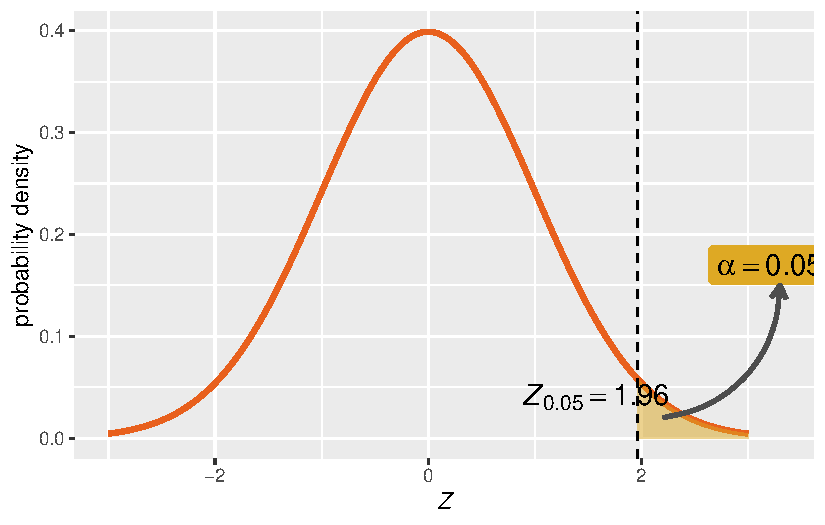
\includegraphics{voorbeelden_files/figure-pdf/fig-normal-1.pdf}

}

\caption{\label{fig-normal}Standard normal distribution with critical
value for \(\alpha = 0.05\).}

\end{figure}%

\begin{Shaded}
\begin{Highlighting}[]
\FunctionTok{library}\NormalTok{(ggplot2)}

\NormalTok{t\_values }\OtherTok{\textless{}{-}} \FunctionTok{seq}\NormalTok{(}\SpecialCharTok{{-}}\DecValTok{3}\NormalTok{, }\DecValTok{3}\NormalTok{, }\AttributeTok{by =} \FloatTok{0.1}\NormalTok{)}
\NormalTok{z\_values }\OtherTok{\textless{}{-}} \FunctionTok{seq}\NormalTok{(}\SpecialCharTok{{-}}\DecValTok{3}\NormalTok{, }\DecValTok{3}\NormalTok{, }\AttributeTok{by =} \FloatTok{0.1}\NormalTok{)}

\NormalTok{dataframe }\OtherTok{\textless{}{-}} \FunctionTok{data.frame}\NormalTok{(}
  \AttributeTok{t =} \FunctionTok{c}\NormalTok{(z\_values, }\FunctionTok{rep}\NormalTok{(t\_values, }\DecValTok{3}\NormalTok{)),}
  \AttributeTok{prob =} \FunctionTok{c}\NormalTok{(}
    \FunctionTok{dnorm}\NormalTok{(z\_values),}
    \FunctionTok{dt}\NormalTok{(t\_values, }\AttributeTok{df =} \DecValTok{1}\NormalTok{),}
    \FunctionTok{dt}\NormalTok{(t\_values, }\AttributeTok{df =} \DecValTok{5}\NormalTok{),}
    \FunctionTok{dt}\NormalTok{(t\_values, }\AttributeTok{df =} \DecValTok{20}\NormalTok{)}
\NormalTok{  ),}
  \AttributeTok{df =} \FunctionTok{factor}\NormalTok{(}
    \FunctionTok{c}\NormalTok{(}
      \FunctionTok{rep}\NormalTok{(}\StringTok{"standard normal"}\NormalTok{, }\FunctionTok{length}\NormalTok{(z\_values)),}
      \FunctionTok{rep}\NormalTok{(}\StringTok{"df = 1"}\NormalTok{, }\FunctionTok{length}\NormalTok{(t\_values)),}
      \FunctionTok{rep}\NormalTok{(}\StringTok{"df = 5"}\NormalTok{, }\FunctionTok{length}\NormalTok{(t\_values)),}
      \FunctionTok{rep}\NormalTok{(}\StringTok{"df = 20"}\NormalTok{, }\FunctionTok{length}\NormalTok{(t\_values))}
\NormalTok{      ),}
    \AttributeTok{levels =} \FunctionTok{c}\NormalTok{(}
      \StringTok{"df = 1"}\NormalTok{, }\StringTok{"df = 5"}\NormalTok{, }\StringTok{"df = 20"}\NormalTok{, }\StringTok{"standard normal"}
\NormalTok{      )}
\NormalTok{    ) }
\NormalTok{  )}

\FunctionTok{ggplot}\NormalTok{(}
\NormalTok{  dataframe, }
  \FunctionTok{aes}\NormalTok{(}
    \AttributeTok{x =}\NormalTok{ t, }\AttributeTok{y =}\NormalTok{ prob, }
    \AttributeTok{group =}\NormalTok{ df, }\AttributeTok{color =}\NormalTok{ df, }\AttributeTok{linewidth =}\NormalTok{ df, }\AttributeTok{linetype =}\NormalTok{ df)}
\NormalTok{  ) }\SpecialCharTok{+}
  \FunctionTok{geom\_line}\NormalTok{(}
\NormalTok{  ) }\SpecialCharTok{+}
  \FunctionTok{scale\_color\_manual}\NormalTok{(}
    \AttributeTok{values =} \FunctionTok{c}\NormalTok{( }\FunctionTok{rep}\NormalTok{(}\StringTok{"black"}\NormalTok{, }\DecValTok{3}\NormalTok{), }\StringTok{"\#e8601d"}\NormalTok{)}
\NormalTok{    ) }\SpecialCharTok{+} 
  \FunctionTok{scale\_linewidth\_manual}\NormalTok{(}
    \AttributeTok{values =} \FunctionTok{c}\NormalTok{(}\DecValTok{1}\NormalTok{, }\DecValTok{1}\NormalTok{, }\DecValTok{1}\NormalTok{, }\FloatTok{1.2}\NormalTok{)}
\NormalTok{  ) }\SpecialCharTok{+}
  \FunctionTok{scale\_linetype\_manual}\NormalTok{(}
    \AttributeTok{values =} \FunctionTok{c}\NormalTok{(}
      \StringTok{"df = 1"}\OtherTok{=}\StringTok{"longdash"}\NormalTok{, }
      \StringTok{"df = 5"}\OtherTok{=}\StringTok{"dashed"}\NormalTok{, }
      \StringTok{"df = 20"}\OtherTok{=}\StringTok{"dotted"}\NormalTok{,}
      \StringTok{"standard normal"}\OtherTok{=}\StringTok{"solid"} 
\NormalTok{    )}
\NormalTok{  ) }\SpecialCharTok{+}
  \FunctionTok{labs}\NormalTok{(}
    \AttributeTok{x =} \FunctionTok{expression}\NormalTok{(}\FunctionTok{italic}\NormalTok{(t)),}
    \AttributeTok{y =} \StringTok{"probability density"}
\NormalTok{  )}
\end{Highlighting}
\end{Shaded}

\begin{figure}[H]

\centering{

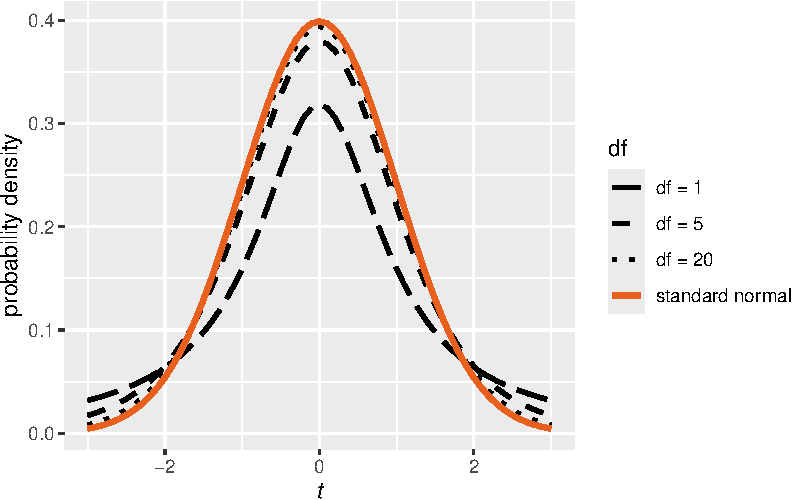
\includegraphics{voorbeelden_files/figure-pdf/fig-tdistributions-1.pdf}

}

\caption{\label{fig-tdistributions}Various \(t\)-distributions and a
normal distribution}

\end{figure}%

\#:::\{.content-visible when-format=``html''\}

\begin{Shaded}
\begin{Highlighting}[]
\FunctionTok{library}\NormalTok{(plotly)}
\NormalTok{p }\OtherTok{\textless{}{-}} \FunctionTok{qplot}\NormalTok{(}\FunctionTok{c}\NormalTok{(}\DecValTok{1}\NormalTok{, }\DecValTok{2}\NormalTok{, }\DecValTok{3}\NormalTok{), }\FunctionTok{c}\NormalTok{(}\DecValTok{4}\NormalTok{, }\DecValTok{2}\NormalTok{, }\DecValTok{4}\NormalTok{))}
\FunctionTok{ggplotly}\NormalTok{(p)}
\end{Highlighting}
\end{Shaded}

\begin{figure}[H]

\centering{

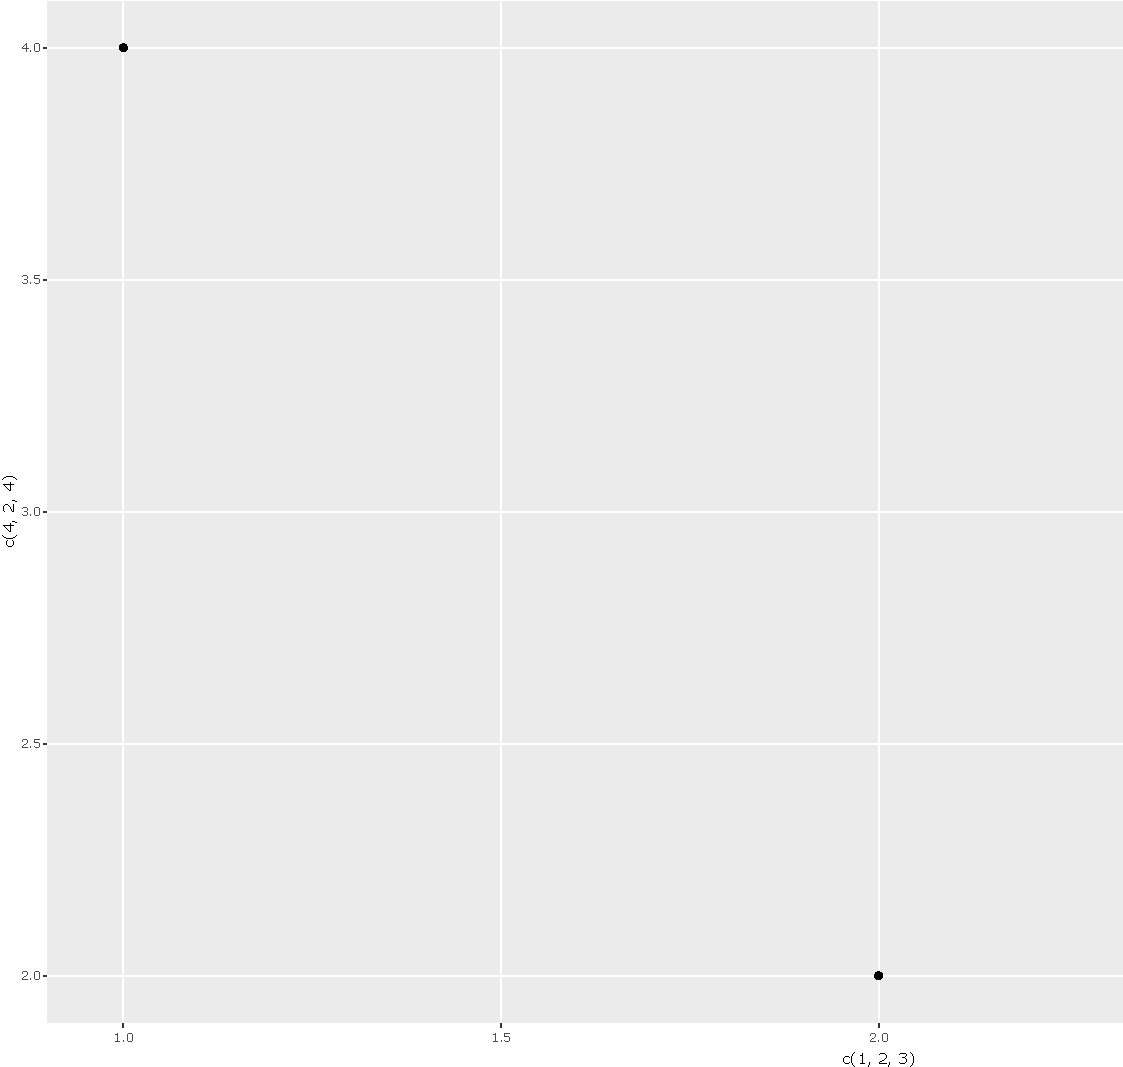
\includegraphics{voorbeelden_files/figure-pdf/fig-plotly-1.pdf}

}

\caption{\label{fig-plotly}test}

\end{figure}%

\#:::

\subsection{Inladen van een simulatie in Javascript die elders gehost
is}\label{inladen-van-een-simulatie-in-javascript-die-elders-gehost-is}

In de html-versie wordt dit getoond:

In de PDF-versie wordt dit getoond:

\begin{figure}[H]

{\centering 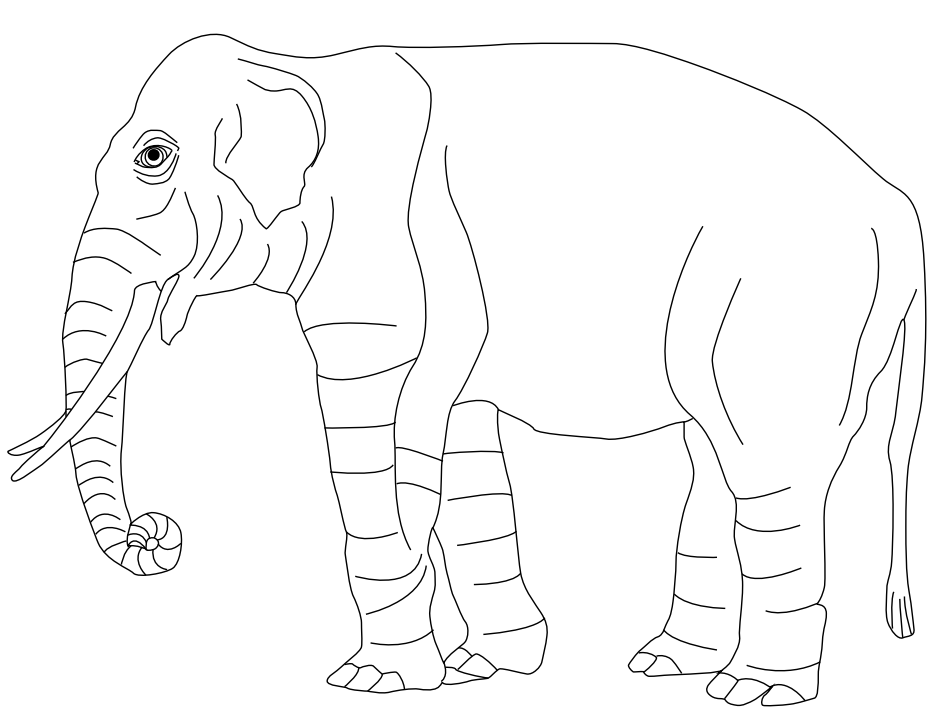
\includegraphics[width=4in,height=\textheight]{./figuren/elephant.png}

}

\caption{Ga naar \url{https://tbb.bio.uu.nl/bvd/simulations/australia/}
voor de simulatie.}

\end{figure}%

\subsection{LaTeX-macros}\label{latex-macros}

In het bestand \_macros.tex kunnen macros worden gedefinieerd. Dat
bestand moet bovenaan ieder document worden ingeladen (zie eerste regel
van dit bestand).

\subsection{Voorbeelden:}\label{voorbeelden}

Voor kansverdelingen heb ik de macro \textbackslash pr\{\}\$
gedefineerd:
\[\textrm{Pr}\!\left(A \cap B\right) = \textrm{Pr}\!\left(A\right) \textrm{Pr}\!\left(B | A\right).\]

\[\textrm{Pr}\!\left(A \cup B\right) = \textrm{Pr}\!\left(A\right) + \textrm{Pr}\!\left(B\right) - \textrm{Pr}\!\left(A \cap B\right).\]

Voor de verwachtingswaarde de macro \textbackslash ev\{\}: \[
\mathbb{E}\!\left(X\right) = \sum_x  x\, \textrm{Pr}\!\left(X = x\right).
\] De differentiaaloperator is \textbackslash diff: \[
\mathbb{E}\!\left(X\right) = \int_{-\infty}^\infty  x\, \textrm{Pr}\!\left(X = x\right)  \mathrm{d}\,x.
\] Voor varianties \textbackslash var\{\}``:

\[
\mathrm{Var}\!\left(X\right)  = \sum_x  \left(x - \mathbb{E}\!\left(X\right)\right)^2 \, \textrm{Pr}\!\left(X = x\right)
\] \[
\mathrm{Var}\!\left(X\right) = \int_{-\infty}^\infty  \left(x - \mathbb{E}\!\left(X\right)\right)^2 \, \textrm{Pr}\!\left(X = x\right) \mathrm{d}\,x.
\]

Voor standaarddeviaties \textbackslash sd\{\}: \[
\sigma\left(X\right) = \sqrt{\mathrm{Var}\!\left(X\right)}.
\]

\subsection{Mermaid}\label{mermaid}

Met Mermaid kun je heel gemakkelijk diagrammen maken:

\begin{figure}

\centering{

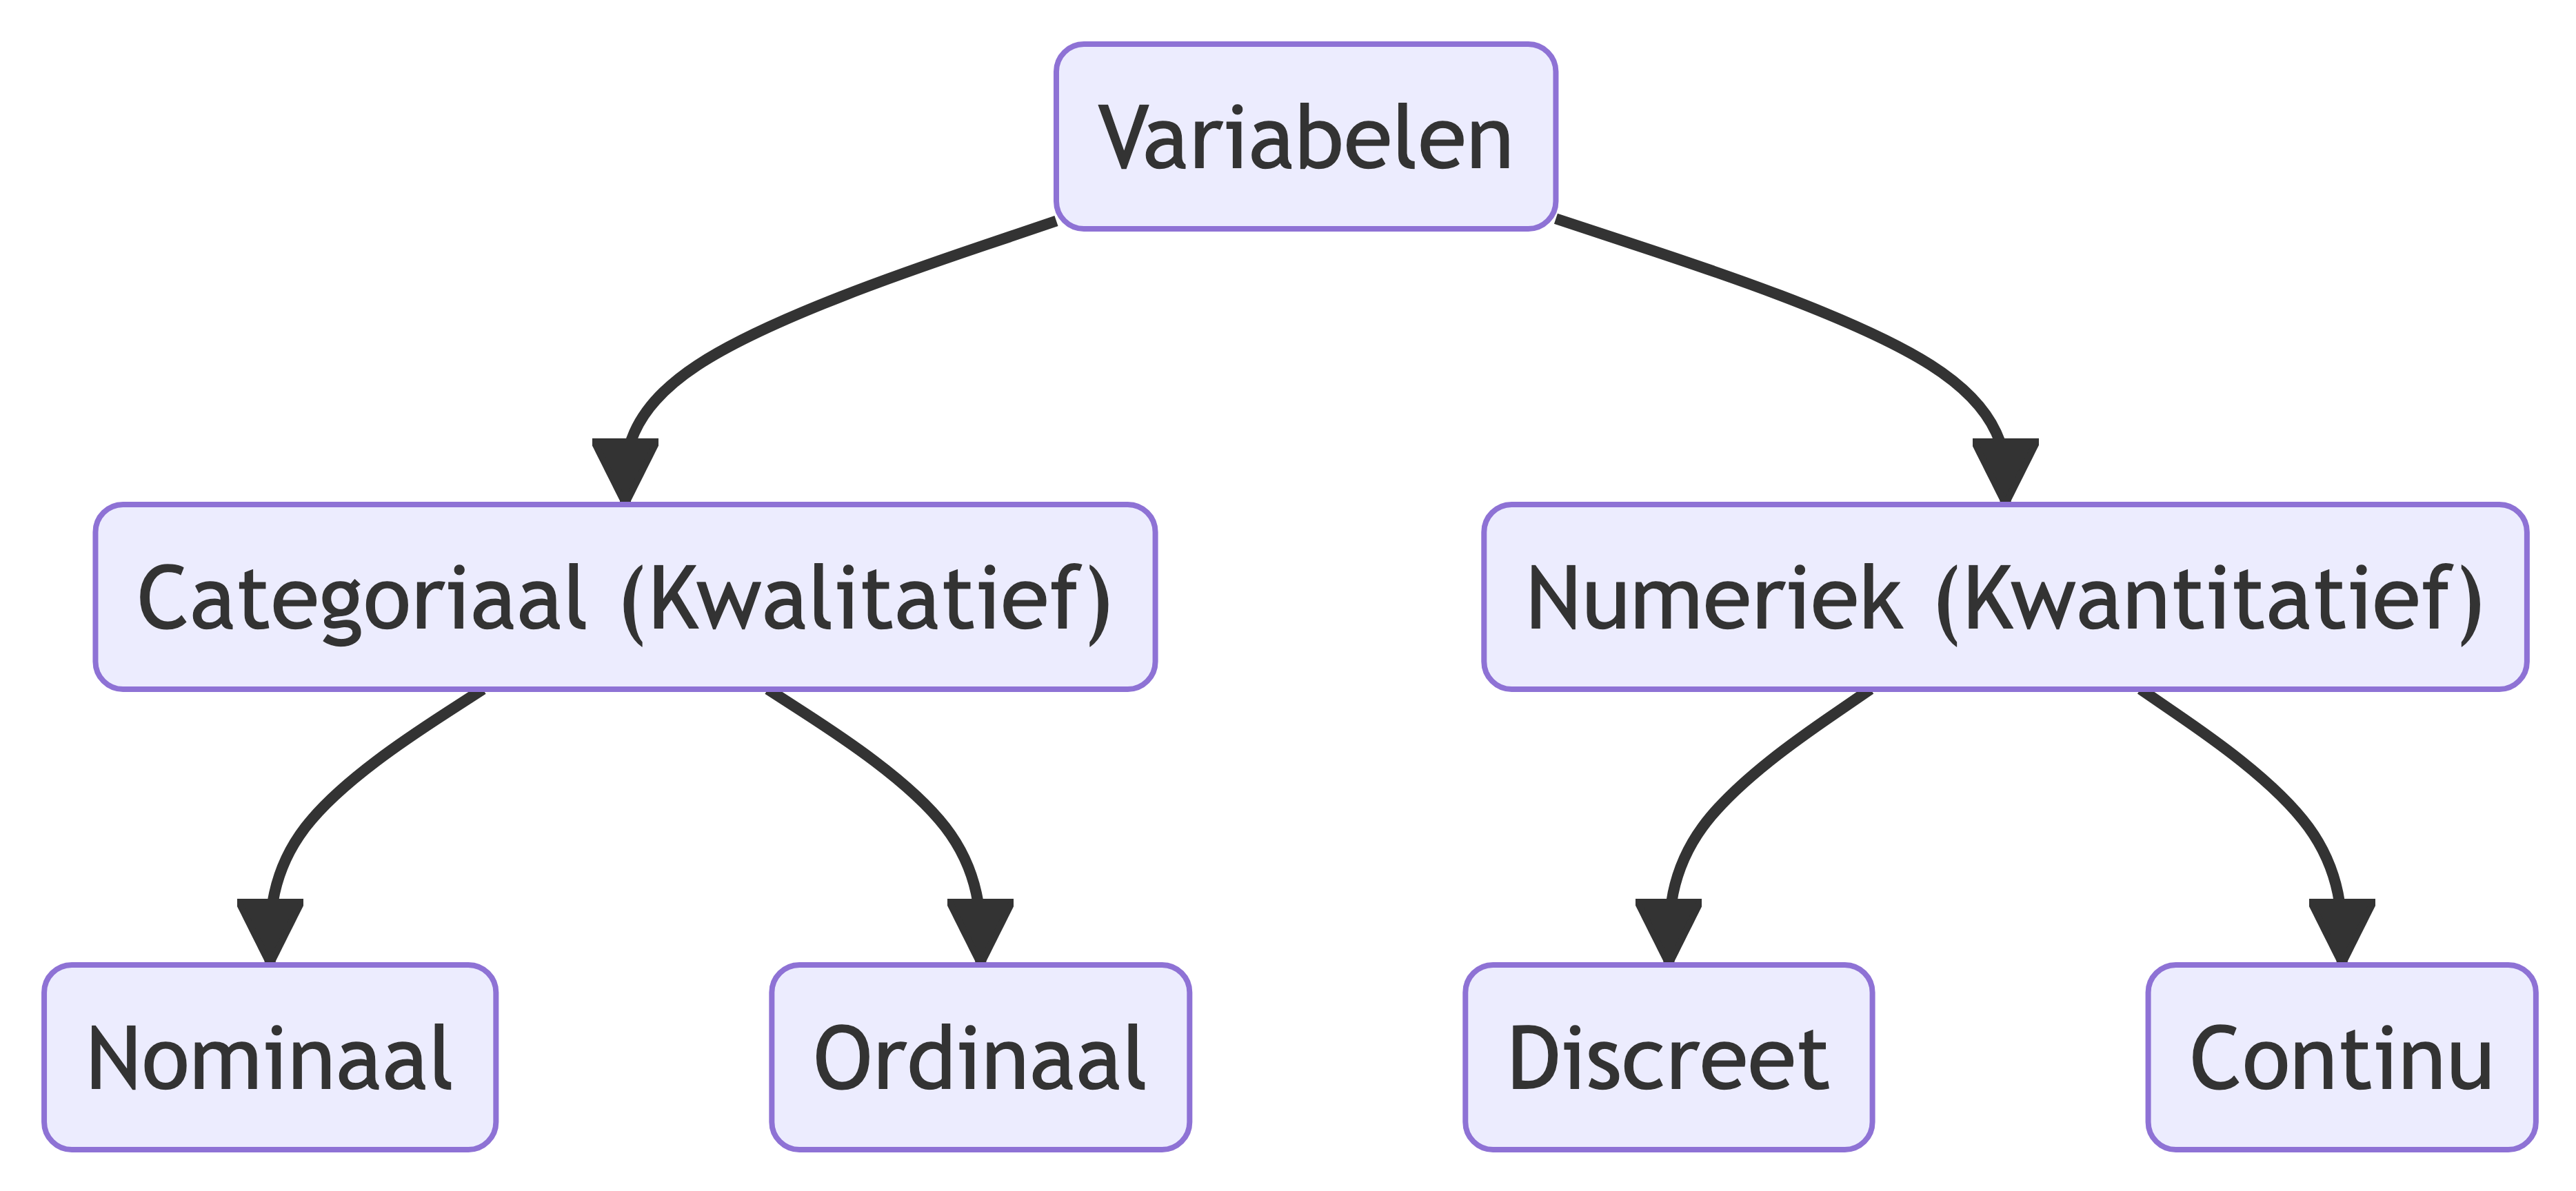
\includegraphics[width=4.87in,height=2.26in]{voorbeelden_files/figure-latex/mermaid-figure-1.png}

}

\caption{\label{fig-variables}}

\end{figure}%

\subsection{Callouts}\label{callouts}

We kunnen gebruik maken van call-outs:

\begin{tcolorbox}[enhanced jigsaw, opacitybacktitle=0.6, colbacktitle=quarto-callout-note-color!10!white, rightrule=.15mm, colback=white, bottomrule=.15mm, title=\textcolor{quarto-callout-note-color}{\faInfo}\hspace{0.5em}{Opmerking}, toprule=.15mm, bottomtitle=1mm, breakable, opacityback=0, colframe=quarto-callout-note-color-frame, titlerule=0mm, coltitle=black, toptitle=1mm, left=2mm, leftrule=.75mm, arc=.35mm]

Note that there are five types of callouts, including: \texttt{note},
\texttt{warning}, \texttt{important}, \texttt{tip}, and
\texttt{caution}.

\end{tcolorbox}

\begin{tcolorbox}[enhanced jigsaw, opacitybacktitle=0.6, colbacktitle=quarto-callout-tip-color!10!white, rightrule=.15mm, colback=white, bottomrule=.15mm, title=\textcolor{quarto-callout-tip-color}{\faLightbulb}\hspace{0.5em}{Tip with Title}, toprule=.15mm, bottomtitle=1mm, breakable, opacityback=0, colframe=quarto-callout-tip-color-frame, titlerule=0mm, coltitle=black, toptitle=1mm, left=2mm, leftrule=.75mm, arc=.35mm]

This is an example of a callout with a title.

\end{tcolorbox}

\begin{tcolorbox}[enhanced jigsaw, opacitybacktitle=0.6, colbacktitle=quarto-callout-caution-color!10!white, rightrule=.15mm, colback=white, bottomrule=.15mm, title=\textcolor{quarto-callout-caution-color}{\faFire}\hspace{0.5em}{Expand To Learn About Collapse}, toprule=.15mm, bottomtitle=1mm, breakable, opacityback=0, colframe=quarto-callout-caution-color-frame, titlerule=0mm, coltitle=black, toptitle=1mm, left=2mm, leftrule=.75mm, arc=.35mm]

This is an example of a `folded' caution callout that can be expanded by
the user. You can use \texttt{collapse="true"} to collapse it by default
or \texttt{collapse="false"} to make a collapsible callout that is
expanded by default.

\end{tcolorbox}

\begin{tcolorbox}[enhanced jigsaw, opacitybacktitle=0.6, colbacktitle=quarto-callout-tip-color!10!white, rightrule=.15mm, colback=white, bottomrule=.15mm, title=\textcolor{quarto-callout-tip-color}{\faLightbulb}\hspace{0.5em}{Tip \ref*{tip-example}: Cross-Referencing a Tip}, toprule=.15mm, bottomtitle=1mm, breakable, opacityback=0, colframe=quarto-callout-tip-color-frame, titlerule=0mm, coltitle=black, toptitle=1mm, left=2mm, leftrule=.75mm, arc=.35mm]

\quartocallouttip{tip-example} 

Add an ID starting with \texttt{\#tip-} to reference a tip.

\end{tcolorbox}

See Tip~\ref{tip-example}\ldots{}

\subsection{How to format questions/problem
sets}\label{how-to-format-questionsproblem-sets}

\begin{exercise}[Test
1]\protect\hypertarget{exr-test1}{}\label{exr-test1}

The equation of any straight line, called a linear equation, can be
written as:

\begin{equation}\phantomsection\label{eq-line}{ 
y = mx + b
}\end{equation}

Je kunt verwijzen naar Vergelijking~\ref{eq-line}, of
Verg.~\ref{eq-line}.

\textbf{a.} Blabla?

\textbf{b.} Of blablabla?

\end{exercise}

\subsection{Data Tables}\label{data-tables}

\begin{Shaded}
\begin{Highlighting}[]
\FunctionTok{library}\NormalTok{(DT)}
\FunctionTok{library}\NormalTok{(datasets)}
\FunctionTok{datatable}\NormalTok{(anscombe, }\AttributeTok{options =} \FunctionTok{list}\NormalTok{(}\AttributeTok{pageLength =} \DecValTok{5}\NormalTok{))}
\end{Highlighting}
\end{Shaded}

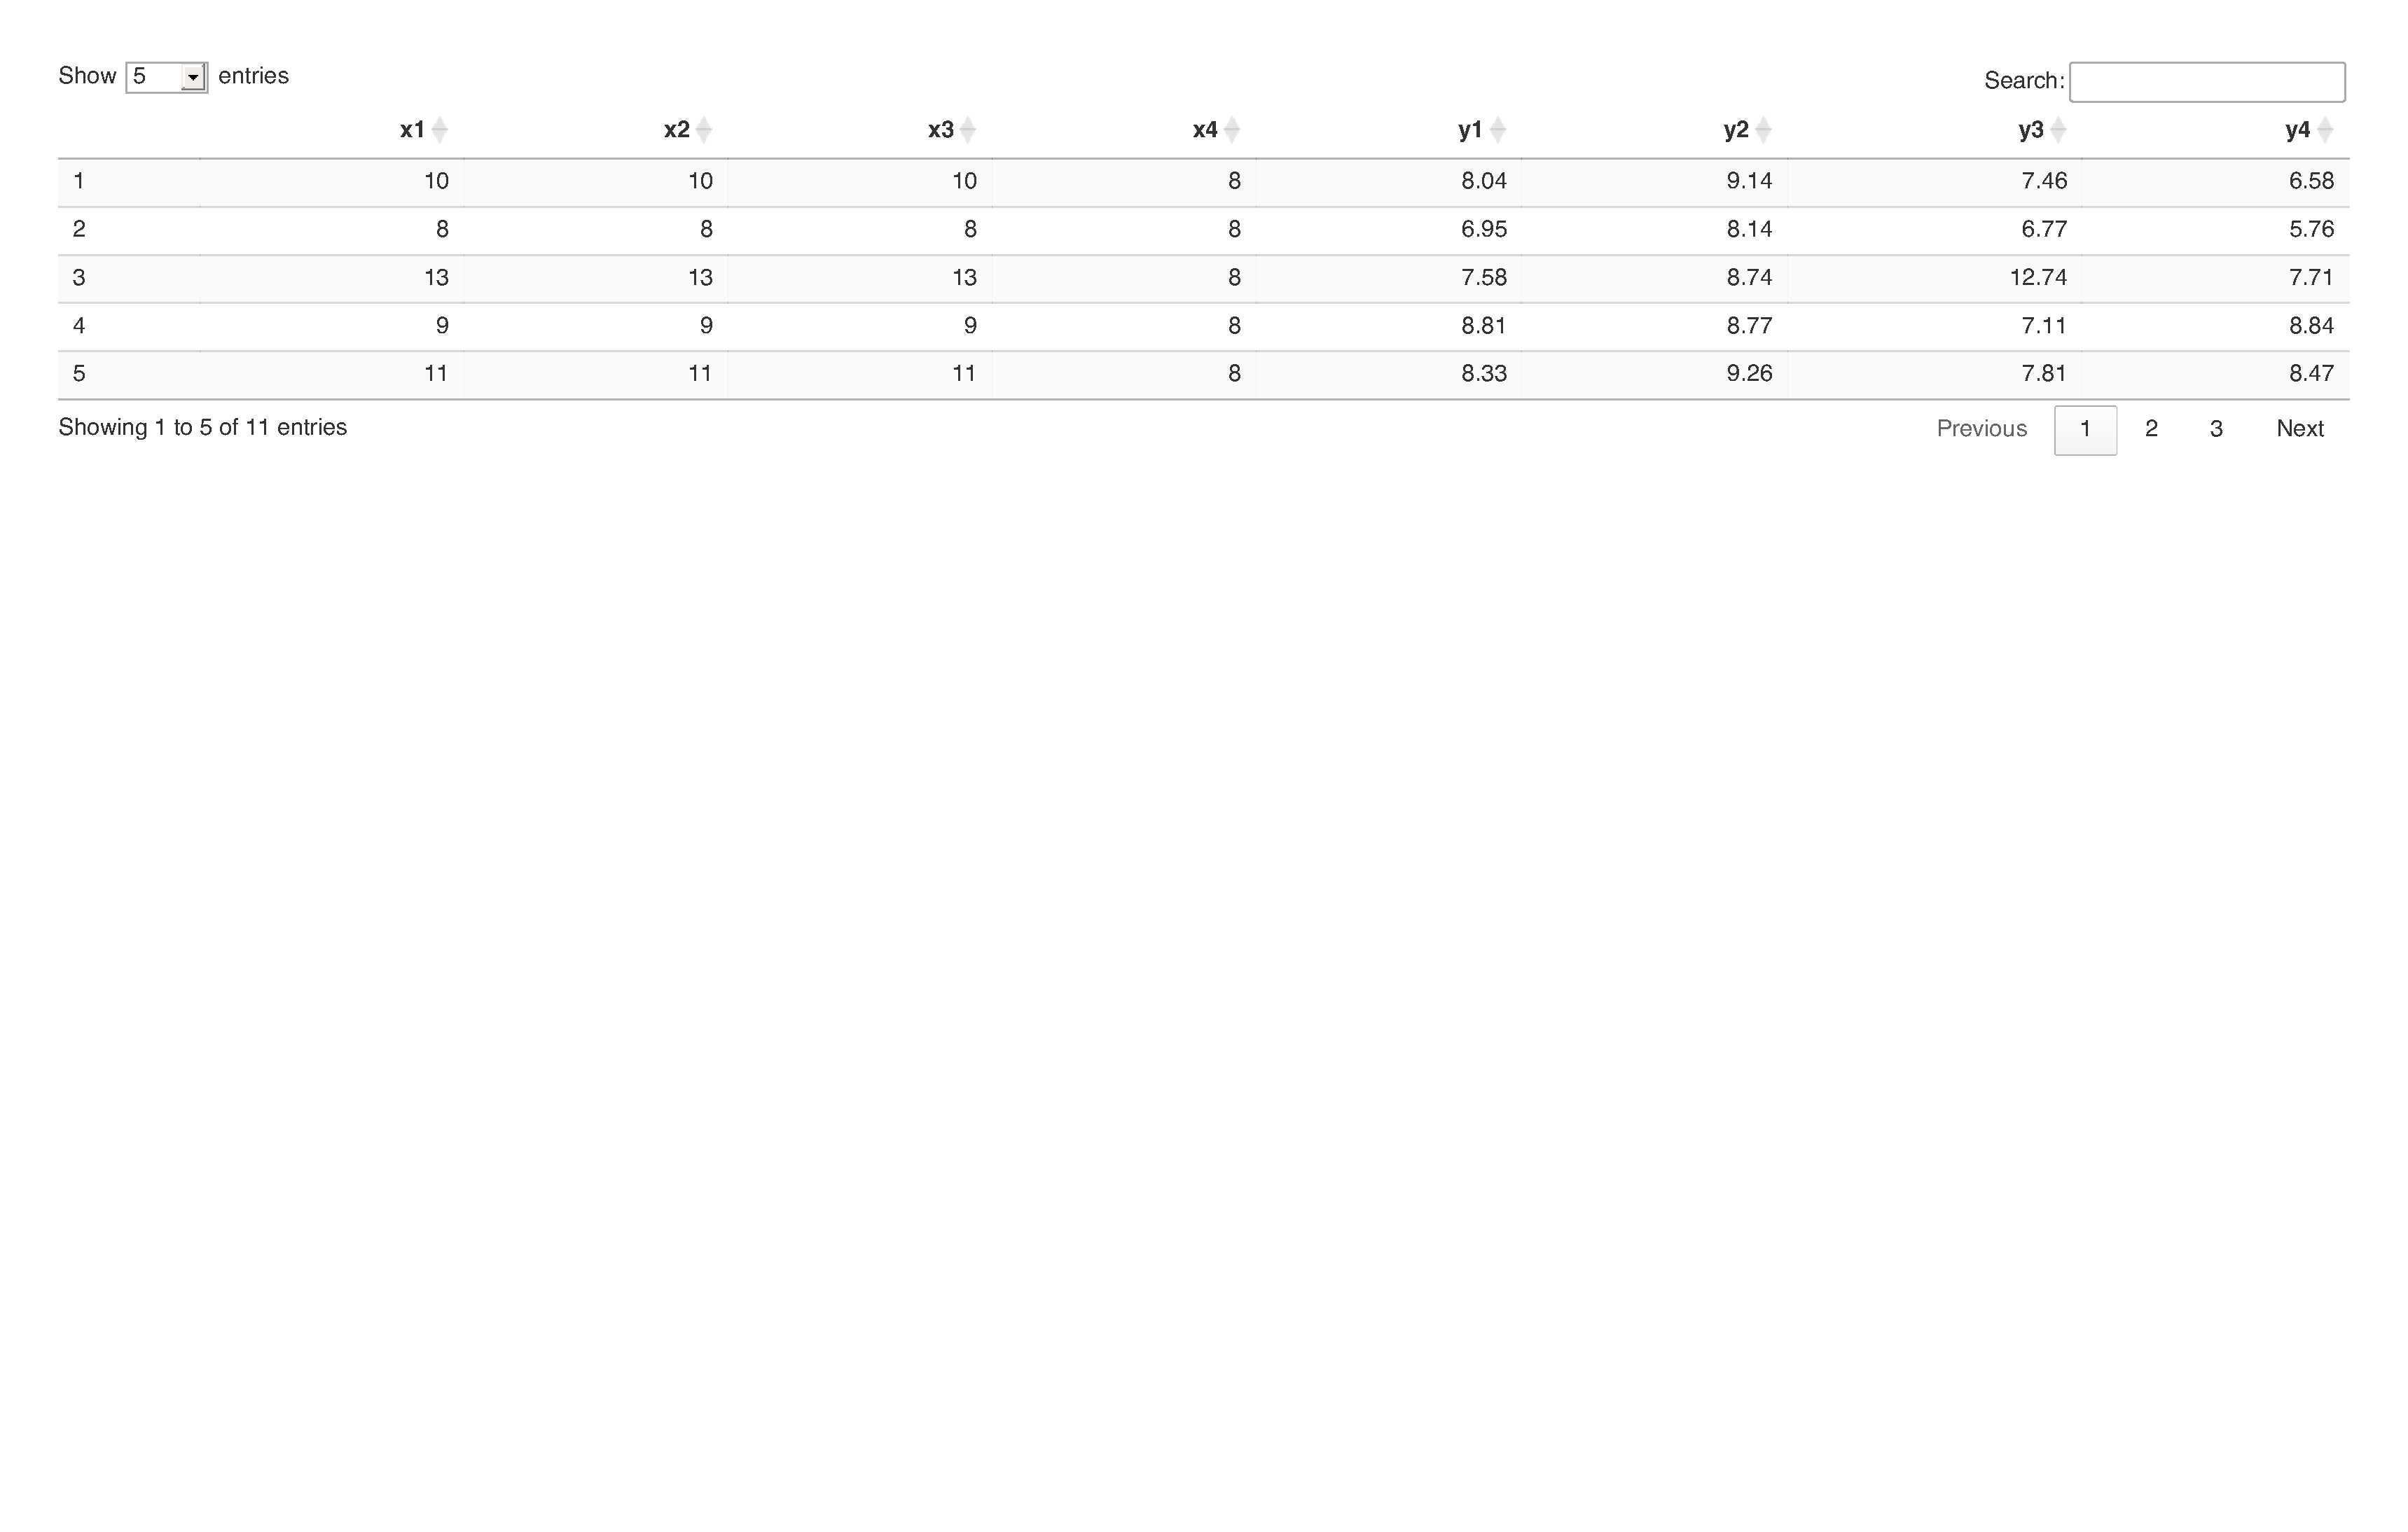
\includegraphics{voorbeelden_files/figure-pdf/tab-anscombe-1.pdf}

\part{Biologische modellering}

\usepackage{libertine}
\addtokomafont{disposition}{\rmfamily}
\renewcommand{\ttdefault}{clmt}

\providecommand{\ped}[1]{_\textrm{#1}}
\providecommand{\ap}[1]{^\textrm{#1}}
\providecommand{\app}[1]{^\textrm{#1}}

\providecommand*{\angs}{\smash{\mathrm{\ring A}}}
\providecommand*{\celsius}{\mathrm{~\circ C}}
\providecommand*{\micro}{\mu}

\providecommand*{\unit}[1]{\textrm{\,#1}}

\providecommand{\E}{\mathrm{e}}
\providecommand{\I}{\mathrm{i}}
\providecommand{\sfrac}[2]{^{#1}/_{#2}}

\providecommand{\conc}[1]{\left[\mathrm{#1}\right]}

\providecommand{\command}[1]{\textsl{#1}}
\providecommand{\out}[1]{\begin{verbatim}#1\end{verbatim}}

\providecommand{\diff}{\mathrm{d}\,}

\providecommand*{\deriv}[3][]{% arguments: order of the derivative(optional), function, variable
    \frac{\diff^{#1}#2}{\diff #3^{#1}}}
\providecommand*{\pderiv}[3][]{% arguments: order of the derivative(optional), function, variable
    \frac{\partial^{#1}#2}
        {\partial #3^{#1}}}

\renewcommand{\vec}[1]{{\boldsymbol #1}}

\providecommand{\cov}[2]{\mathrm{Cov}\!\left(#1, #2\right)}
\providecommand{\var}[1]{\mathrm{Var}\!\left(#1\right)}

\providecommand{\mean}[1]{\overline{#1}}

\providecommand{\sd}[1]{\sigma\left(#1\right)}
\providecommand{\ev}[1]{\mathbb{E}\!\left(#1\right)}
\providecommand{\pr}[1]{\textrm{Pr}\!\left(#1\right)}

\begin{figure}

\centering{

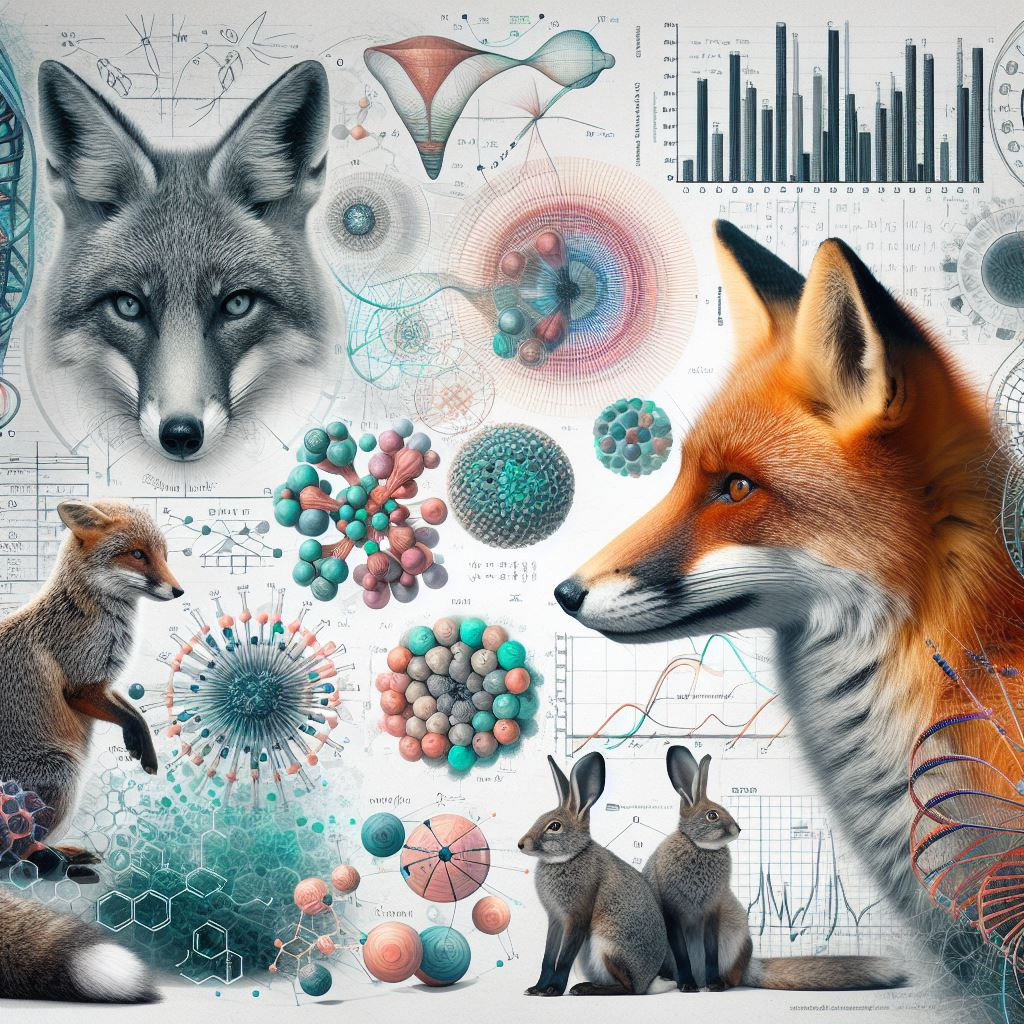
\includegraphics{Modellering/figuren/AI_models.jpeg}

}

\caption{\label{fig-AI_models}Modellering in de biologie, illustratie
gegenereerd door AI. (DALL-E 3, maart 2024)}

\end{figure}%

\chapter{Modellen in de biologie}\label{modellen-in-de-biologie}

\part{Statistiek voor biologen}

\begin{figure}

\centering{


\includegraphics{Statistiek/figuren/AI_statistics.jpeg}

}

\caption{\label{fig-AI_statistics}Statistiek voor biologien, illustratie
gegenereerd door AI. (DALL-E 3, maart 2024)}

\end{figure}%

\chapter{Wat is statistiek?}\label{wat-is-statistiek}

\section{bla}\label{bla}

\cleardoublepage
\phantomsection
\addcontentsline{toc}{part}{Bijlagen}
\appendix

\chapter{Eerse appendix}\label{eerse-appendix}




\end{document}
